\documentclass{acm_proc_article-sp}

\usepackage[utf8]{inputenc}
\usepackage[T1]{fontenc}
\usepackage[activate=compatibility]{microtype}

% autoref command
\usepackage[pdftex,urlcolor=black,colorlinks=true,linkcolor=black,citecolor=black]{hyperref}
\def\sectionautorefname{Section}
\def\subsectionautorefname{Subsection}
\def\subfloatautorefname{Subfigure}

\usepackage[lofdepth,lotdepth]{subfig}
\usepackage{enumitem}
\usepackage{textcomp}
\usepackage{mathtools}
\usepackage{url}

% give emph a normal fontsize
\let\oldemph\emph
\renewcommand{\emph}[1]{\oldemph{\fontsize{9}{9}\selectfont #1}}

% more readable footnote layout
\renewcommand{\footnotesize}{\fontsize{8pt}{10pt}}
\setlength{\footnotesep}{.5cm}

% todo macro
\usepackage{color}
\newcommand{\todo}[1]{\noindent\textcolor{red}{{\bf \{TODO}: #1{\bf \}}}}

% listings and Verbatim environment
\usepackage{fancyvrb}
\usepackage{relsize}
\usepackage{listings}
\usepackage{verbatim}
\newcommand{\defaultlistingsize}{\fontsize{8pt}{9.5pt}}
\newcommand{\inlinelistingsize}{\fontsize{8pt}{11pt}}
\newcommand{\smalllistingsize}{\fontsize{7.5pt}{9.5pt}}
\newcommand{\listingsize}{\defaultlistingsize}
\RecustomVerbatimCommand{\Verb}{Verb}{fontsize=\inlinelistingsize}
\RecustomVerbatimEnvironment{Verbatim}{Verbatim}{fontsize=\defaultlistingsize}
\lstset{frame=lines,captionpos=b,numberbychapter=false,escapechar=§,
        aboveskip=0.5em,belowskip=0em,abovecaptionskip=0em,belowcaptionskip=0em,
framexbottommargin=-1em,
        basicstyle=\ttfamily\listingsize\selectfont}

\usepackage{color}
\definecolor{lightgray}{rgb}{.9,.9,.9}
\definecolor{darkgray}{rgb}{.4,.4,.4}
\definecolor{purple}{rgb}{0.65, 0.12, 0.82}

\lstdefinelanguage{JavaScript}{
  keywords={typeof, new, true, false, catch, function, return, null, catch, switch, var, if, in, while, do, else, case, break},
  keywordstyle=\color{blue}\bfseries,
  ndkeywords={class, export, boolean, throw, implements, import, this},
  ndkeywordstyle=\color{darkgray}\bfseries,
  identifierstyle=\color{red},
  sensitive=false,
  showstringspaces=false,
  comment=[l]{//},
  morecomment=[s]{/*}{*/},
  commentstyle=\color{purple}\ttfamily,
  stringstyle=\color{gray}\ttfamily,
  morestring=[b]',
  morestring=[b]"
}

% use Courier from this point onward, except for URLs
\let\oldttdefault\ttdefault
\renewcommand{\ttdefault}{pcr}
\let\oldurl\url
\renewcommand{\UrlFont}{\fontfamily{\oldttdefault}\selectfont}

% linewrap symbol
\definecolor{grey}{RGB}{130,130,130}
\newcommand{\linewrap}{\raisebox{-.6ex}{\textcolor{grey}{$\hookleftarrow$}}}

% for 1st, 2nd, etc. superscripting
\newcommand{\ts}{\textsuperscript}

% more pleasing quote environment
\usepackage{tikz}
\newcommand*{\openquote}{\tikz[remember picture,overlay,xshift=-7pt,yshift=1pt]
     \node (OQ) {\fontfamily{fxl}\fontsize{16}{16}\selectfont``};\kern0pt}
\newcommand*{\closequote}{\tikz[remember picture,overlay,xshift=2pt,yshift=-4.5pt]
     \node (CQ) {\fontfamily{fxl}\fontsize{16}{16}\selectfont''};}
\renewenvironment{quote}%
{\setlength{\parindent}{1cm}\par\openquote}
{\closequote\vspace{-4.5pt}
}

\begin{document}

\title{NiteOutMag\hspace{-1.5pt}\raisebox{6pt}{$^\textbf{\sffamily TM}$}---At Least the Web\\ Remembers What Happened Last Night}

\numberofauthors{2}
\author{
% Tom, Ruben, Raphaël, Giuseppe, José
}
\maketitle

\begin{abstract}
The chorus of the popular song \emph{Tik Tok} by the artist \emph{Ke\$ha} goes
\emph{``Don't stop, make it pop. DJ, blow my speakers up. Tonight, I'mma fight.
'Til we see the sunlight. Tik tok on the clock. But the party don't stop, no.''}
We all know, however, that each party comes to an end eventually.
With NiteOutMag\texttrademark, we present a~Chrome Web application
that can help people recover what (the hell) happened last night.
Among the younger generation, nightlife activities---just about like any other
activity---together with related multimedia data get shared online on social networks.
The problem is that for one and the same event, the event-related user-generated data
may be shared on a~plethora of social networks.
Therefore, for this challenge, we introduce an application
that leverages event data from several event databases,
social data from multiple social networks, and media data from some media platforms.
The collected data for events around a~given area is then compiled
in an event-centric magazine-like way, where each page represents one event.
Just like the nightlives of people happen \emph{ad hoc} from one party to the other,
the NiteOutMag\texttrademark~application as well
gathers all its data on-the-fly, without the burden of pre-compiled data directories.
The application is available online\footnote{\url{http://goo.gl/bXM8f}}.
A~screencast showcasing the application is also available\footnote{\url{https://t.co/3R8h2RnW}}.
\end{abstract}

%\category{H.3.4}{Information Systems}{Information Storage and Retrieval}[World Wide Web]
%\category{H.3.5}{Online Information Services}{Web-based services}

%\keywords{}

\section{Introduction}
%missing: event extraction, event posts aggregation
In March 2012, the at the time 901 million monthly active users
of the social networking site (SNS) Facebook
have uploaded more than 300 million photos on average per day~\cite{Facebook2012}.
Many of those photos are event-related, \emph{e.g.},
illustrate events like music concerts that a~social network user has attended.
Facebook, however, albeit the biggest, is only one among a~plethora of social networks
that event attendants may have shared their event-related content on.
In the next subsection, we thus list the SNSs considered for
NiteOutMag\texttrademark.

\subsection{Social Networks} \label{sec:social-networks}
A~social network is an online service or media platform that focuses on building
and reflecting social relationships among people sharing interests and/or activities.
In this paper, we consider eleven different social networks
that represent all together most of the Western world's market share.
In detail, the considered social networks are
\mbox{Google+} (\url{google.com/+}),
Myspace (\url{myspace.com}),
Facebook (\url{facebook.com}),
Twitter ({twitter.com}),
Instagram (\url{instagram.com}),
Flickr (\url{flickr.com}),
YouTube (\url{youtube.com}),
yfrog (\url{yfrog.com}),
MobyPicture (\url{mobypicture.com}),
Twitpic (\url{twitpic.com}), and
\mbox{img.ly} (\url{img.ly}).

The actual detection of events based on information from SNSs
is out of bounds for this paper.
We point the reader to, \emph{e.g.},~\cite{Petkos2012} by Petkos \emph{et al.},
which is a~typical example of event detection based on multimodal clustering.
For our purposes, event databases as listed below are adequate.

\subsection{Event Databases}
An event database is an online service that holds metadata
for a~categorized set of events that can be queried programmatically.
We consider four event databases, namely
Eventful (\url{eventful.com}),
Foursquare (\url{foursquare.com}),
Upcoming (\url{upcoming.org}), and
Google Places (\url{google.com/places}).

\section{Related Work}
Capture life moments and tell them using social networks is addressed in~\cite{Atosy2011}, where the authors investigated about the interaction between event stories and the use of social networks to tell them. They proposed Storify~\cite{Storify2012}, a web application which guides and assists designers in the concept generation stage by providing assistance in: (1) sorting and organizing the items of an experience similar to the elements of a story, (2) communicating and discussing strategies on how to guide a user towards an intended experience. The overall storytelling creation is supervised by the user, who describes the story as a crafted experience~\cite{Hassenzahl2010}. Streams of news navigate through the social platforms such as Twitter, YouTube. Getting the big picture from them is the objective of Storyful~\cite{Storyful2012}. This application allows the user to navigate through the story created by other users or to create his own aggregating the content available from Twitter, Youtube and adding more. 
Events have a key role in the human life and illustrating events with media items stemming from social networks is an active topic of research since the rise of social networking. In~\cite{Brenner2012}, Brenner and Izquierdo present an approach to detect social events and retrieve associated photos in collaboratively annotated photo collections combining data of various modalities such as time, location, and textual and visual features. In~\cite{Liu2011}, Liu \emph{et al.} present a method for combining semantic inferencing and visual analysis for automatically gathering photos and videos illustrating events. Regarding esthetic aspects of media compilation, in~\cite{Sandhaus2011}, Sandhaus \emph{et al.} consider visual and esthetic features for the automatic creation of photo books. Obrador \emph{et al.}\ use visual and esthetic features for a~category-based approach to automatically assess the esthetic appeal of photographs~\cite{Obrador2012}.

\section{Implementation}
In this section, we provide implementation details for the
NiteOutMag\texttrademark application.
It is implemented as a~Chrome application, as this technique provides
a transparent statement about the required resources of the application,
\emph{i.e.}, cross-domain access to event databases and search APIs.

\subsection{Geocoding}
The application focuses on events that occurred in a~certain area.
While event databases tend to work based on concrete points like
\mbox{(40.7590110, -73.98447220)}, \emph{i.e.},
latitude and longitude pairs, human beings use more human-friendly place references
like \emph{Times Square, New York}.
Geocoding is the process of finding associated geographic coordinates
(often expressed as latitude and longitude) from other geographic data,
such as street addresses, or zip codes.
The user can enter an exact address, such as
\emph{618 W. 46th St, New York, NY 10036}, or a~very broad area like \emph{Las Vegas}.
The returned latitude and longitude pair is always the center
of the particular point or area of interest.
In our implementation, we use the Google Geocoding API~\cite{Geocoding2012}.

\subsection{Event Search}
Based on a~latitude and longitude pair, we search the before-mentioned
event databases via their respective event search
APIs~\cite{Eventful2012,Foursquare2012,GooglePlaces2012,Upcoming2012}
for \emph{past} events within an empirically determined radius of five kilometers.
We sanitize the event titles by removing HTML tags, punctuation,
common abbreviations (like \emph{w/}, which becomes \emph{with}, or \emph{ft./feat.},
which becomes \emph{featuring}).
As all events are geographically close, we deduplicate the returned set of events
based on the simple, yet effective Levenshtein distance
with an empirically determined editing distance of five,
which catches things like \emph{Titanic} and \emph{Titanic 3D} for, \emph{e.g.}, movie events.

\subsection{Media Search} \label{sec:media-search}
Unlike event search, media search in our application is \emph{not} based on geolocation.
According to a~study performed in May 2012 by Seline~\cite{Quora2012},
only roughly 1\% of all microposts on Twitter are geotagged.
In addition to that, as our approach covers more SNSs than Twitter,
we need to consider that not all SNSs support geotagging of content.
In consequence, we use a~two-tier approach for media search,
illustrated by a~real event of a~Beach Boys
concert\footnote{\url{http://www.thebeachboys.com/\#tour}}
in the Merriweather Post Pavilion in Columbia, MD.
The event name is \emph{Beach Boys},
the venue name is \emph{Merriweather Post Pavilion},
and the area is \emph{Columbia, Maryland (MD)}.
We define as \emph{human-friendly address}
the first part up to the comma of the \texttt{formatted\_address} field
in the Google Geocoding API~\cite{Geocoding2012},
\emph{i.e.}, \emph{Columbia} in the concrete case.
Human beings aware of the local context do not need to disambiguate, \emph{i.e.},
there is no need to explicitly state \emph{MD}.
The two-tier approach consists thus of a~full-text search for:

\emph{(i)} the (event name) $+$ the (venue name), and

\emph{(ii)} the (event name) $+$ the (human-friendly address).

We have implemented a~media collector consisting of media extractors for all SNSs
listed in \autoref{sec:social-networks}.
% DOUBLE-BLIND REVIEW
% This media collector was first described in~\cite{Khrouf2012}.
% DOUBLE-BLIND REVIEW
It takes a~search term as input, \emph{e.g.},
\emph{Beach Boys Columbia} for the example above,
and then performs a~parallel full-text search using the search APIs of all SNSs.
When all the media extractors have responded, a~unified SNS-agnostic output is delivered.
We propose a~common alignment schema, illustrated in
\autoref{lst:media}, which shows the resulting metadata for an exemplary media item.
\autoref{fig:architecture} shows the overall architecture of the media collector.

\begin{lstlisting}[language=JavaScript,caption={Sample output of the media collector showing a~\mbox{Google+} post (edited for legibility, URLs shortened).},label={lst:media}]
{
  "mediaurl": "http://t.co/ubagkiR9",
  "storyurl": "https://t.co/dau5pBWD",
  "message": {
    "text": "My wife, who once said her vision of
        heaven was being on the lawn bouncing
        around beach balls at a Beach Boys
        concert [...]
        <a href=\"http://t.co/pH2OV1fW\" >
        http://t.co/pH2OV1fW</a> [...]",
    "clean": "My wife, who once said her vision of
        heaven was being on the lawn bouncing
        around beach balls at a Beach Boys
        concert [...]"
  },
  "user": "https://t.co/gIf2UVZR",
  "type": "photo",
  "timestamp": 1329342797000,
  "published": "2012-02-15T21:53:17.000Z"
}
\end{lstlisting}

\begin{figure*}[htb!]
\centering
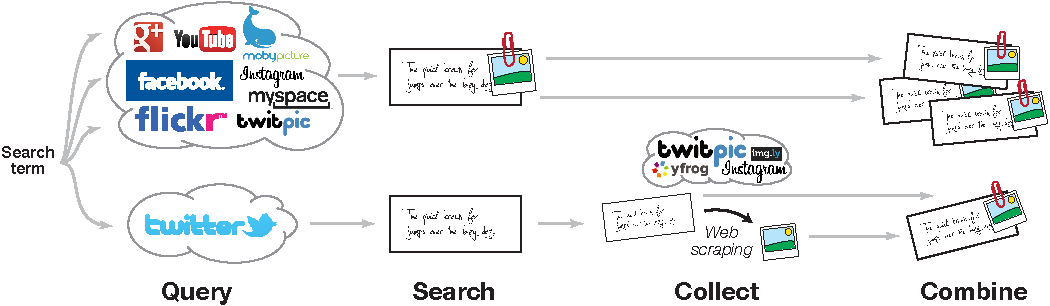
\includegraphics[width=0.8\linewidth]{./architecture.pdf}
\caption{Overview of the media collector: hybrid approach for the media item extraction process using a~combination of API access and Web scraping}
\label{fig:architecture}
\end{figure*}

\subsection{Magazine Layout}
In order to create the illusion of a~real magazine,
flipping from page to page needs to be as credible as possible.
The open-source library turn.js by Emmanuel García~\cite{TurnJs2012}
allows for the dynamic creation of magazines solely based on HTML5 technologies
with a~very realistic page flip effect.
We treat each event as one page of the magazine,
add the event metadata as headline and subheading of the page,
and arrange the images and accompanying microposts to fill the page.
For each event, we use the image with the highest resolution
as background image of the page in order to create a~lifestyle magazine appearance.
For additional print-like look and feel, we use drop caps,
as can be seen in \autoref{fig:screenshot}.
The title page gets dynamically created based on a~Google image search
for the (human-friendly address) $+$ the keyword (nightlife).

\subsection{Installation Instructions}
The NiteOutMag\texttrademark application requires the Chrome browser.
Download the application from the URL \url{http://goo.gl/bXM8f} to the local file system.
Once there, drag and drop it into the \url{chrome://chrome/extensions/} page in the browser.
When you drop it on the extensions page, you will notice an install option popping up there.
When you agree to install, you will see the standard installation dialog
that informs you about the rights that the application is requesting.
It needs access to the before-mentioned event databases and media search APIs.

\section{Experiments}
We have evaluated our application with the top ten list of
United States cities by
population\footnote{\url{http://en.wikipedia.org/wiki/List_of_United_States_cities_by_population}}
with promising results.

\begin{figure}[b!]
\centering
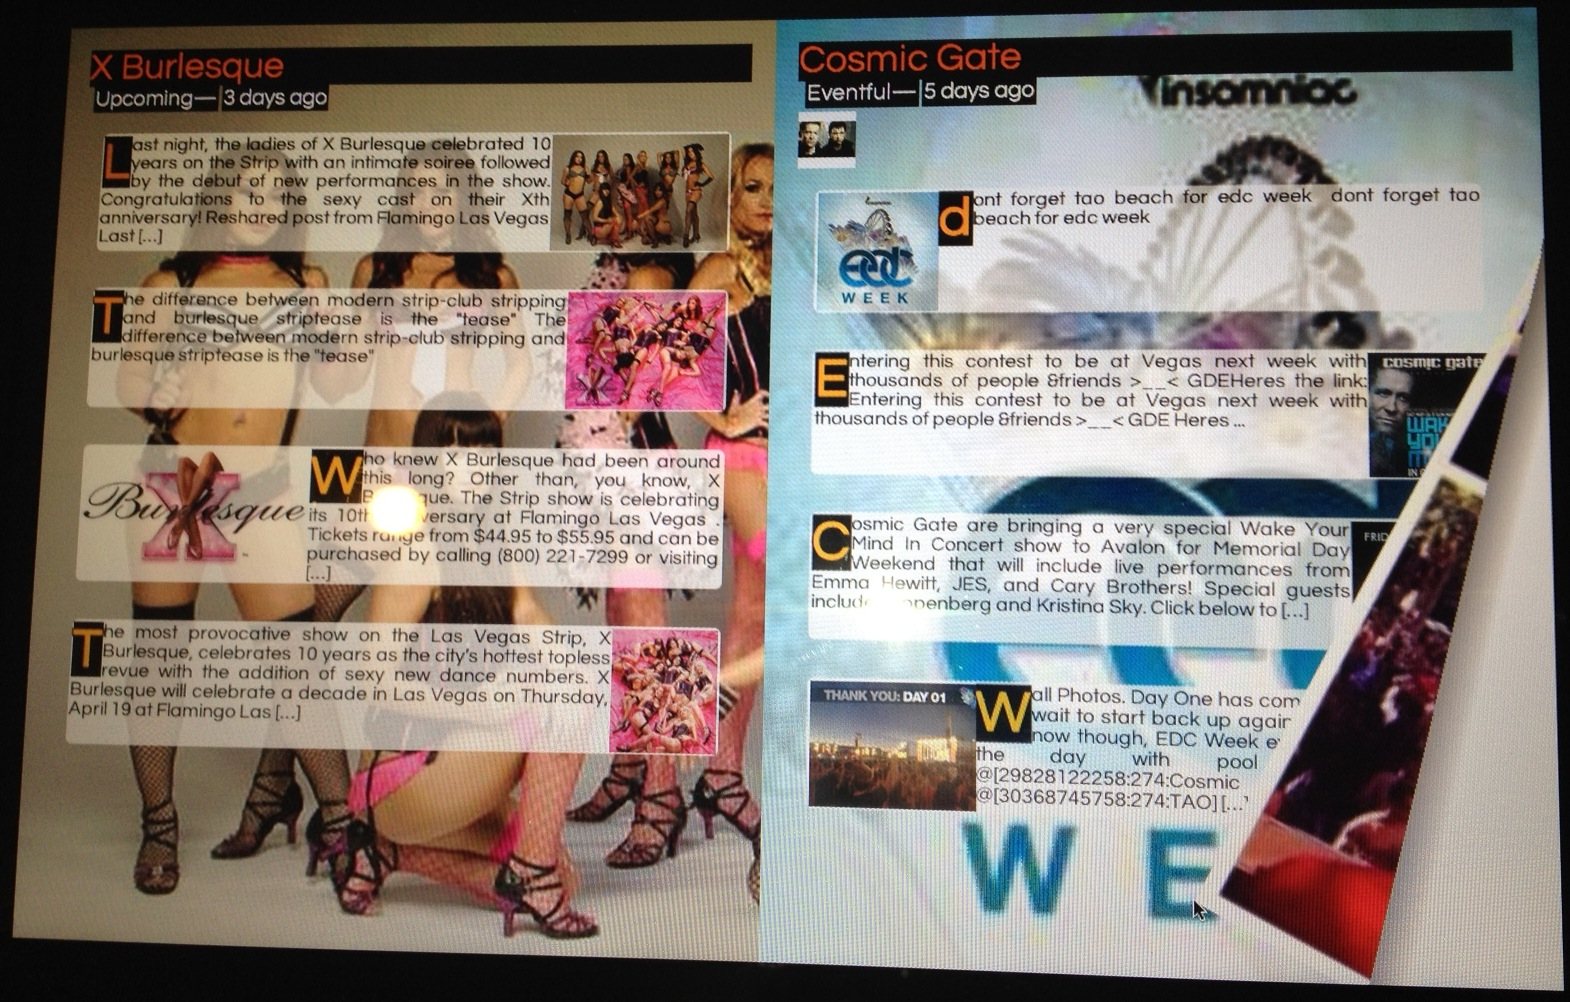
\includegraphics[width=1.0\columnwidth]{./screenshot.jpg}
\caption{Screenshot of the NiteOutMag\texttrademark application with two events from Las Vegas and the righthand-side page about to be flipped}
\label{fig:screenshot}
\end{figure}

\subsection{Query Examples}
In general, big cities and well-known places of interest
reveal good results due to the high density of events.
Popular examples are among others
(\emph{Fisherman's Wharf, San Francisco}),
(\emph{Times Square, New York}),
(\emph{Piccadilly Circus, London}),
or simply (\emph{Ibiza}).	
A~manually compiled list of America's top party cities
from the magazine Maxim\footnote{\url{http://www.maxim.com/movies/americas-top-10-party-cities}}
also reveals interesting results.

\subsection{Discussion and Future Work}
The results stand and fall with the quality of the events
in the event databases.
One problem are stuffed event titles like
\emph{Kandyland 2012 @ the Playboy Mansion -- 1.877.VIP.MANS\-ION}\footnote{\url{http://t.co/YUm7FtmE}},
where the actual event title gets combined with the venue name
and a~vanity contact phone number.
Detection of such stuffed titles is difficult and needs more work.

Event deduplication is a~second issue.
The two movie events \emph{The Avengers} and
\emph{Marvel's The Avengers 3D} are the same for a~human being,
however, for a~machine, the duplication is harder to detect.
Media item deduplication is a~task that we have left for future work.

The system's response time is improvable.
The main issue here is the browser-enforced maximum number
of simultaneous HTTP requests.
With our current four event sources that we have limited
to ten events per source, we already have up to forty events
that we need to search media items for.
As outlined before in \autoref{sec:media-search},
we have opted for a~two-tier approach in order to improve the recall,
which effectively means two search requests per event.
Assuming that for each search request we get on average only two media items,
we have roundabout $5+40*2*2=165$ HTTP requests for only one magazine.
We will investigate ways to improve the application's responsiveness
in the future.

\section{Conclusion}
In this paper, we have reported on a~Chrome Web application that
illustrates events via four event databases and eleven SNSs.
The application harvests event-related data on-the-fly for
a~user-determined center of interest and compiles the data
in an esthetic lifestyle magazine-like way.
Via popular party destinations, big cities, and places of interests,
we have evaluated the retrieved results for both relevancy and
visual appeal, with a~special focus on optimized recall.
While there are actionable issues for future work,
we are quite happy with the outcome so far.

% \section{Acknowledgments}
% Double-blind review process, need to remove for now

\bibliographystyle{abbrv}
\bibliography{acm2012grandchallenge}

\balancecolumns
\end{document}
